\chapter{Implementation}
In this chapter we will explain how is our demo game implemented. We will talk about how are data represented and how different modules and third party software libraries work together.

After consideration of different approaches implemented in games and also proposed efficient solutions to the problem of real-time destructible environment, we decided to try to implement a new approach. We will borrow already tried techniques and put them together in a different way.

Our approach is mostly similar to \emph{Geomod} (described in \cref{sec:common}) with a key differences. Our approach generates Voronoi cell at the point of collision. Then the difference of original mesh and Voronoi cell is calculated and represents damaged object. To generate the debris the intersection of original mesh and Voronoi cell is calculated. This effectively cuts the object into two or more pieces, all of which are put back into simulation and can be damaged again.

Randomization of the size and shape of Voronoi cell guarantees different result after every collision and makes the game look more realistic. The generation of Voronoi cell takes place in closed cube with its centre in the point of collision. In the cube random points are generated in addition to centre one, and the Voronoi cell is the cell of centre point cut by sides of the cube if necessary.

We also considered implementation based on \emph{A fast method for simulating destruction and the generated dust and debris} (see \cref{sec:edem}). Using the same technology as for our demo game, we set up a cube divided into 439 tetrahedrons. After introducing constraints to hold the elements together we experienced drop from default 60fps (set as upper limit) to 13fps. This result is consistent with results in the article~\cite{edem} and the conclusion is that this approach is not suitable for our work.

\section{Program Structure}
The program is running in three threads (\cref{fig:threads}): main thread, threat for subtracting meshes (\cref{sec:subtraction}) and thread for decomposing triangular mesh into set of convex shapes (\cref{sec:decomposition}). Both subtraction and decomposition threads communicate only with main thread and all communication is done in producer-consumer model. Disregarding the initialization, the program runs in following steps:
\begin{enumerate}
\item Perform a step in physics simulation. We measure the time since last step and leave this task entirely to Bullet physics engine.
\item Handle collisions, see \cref{sec:collisions}.
\item Read user input and then apply correct forces to controlled vehicle.
\item Render current state of objects. In this step, graphical representation of every object is updated to comply with its rigid body version. Also the camera has to be properly moved and rotated.
\end{enumerate}

\begin{figure}
        \centering
        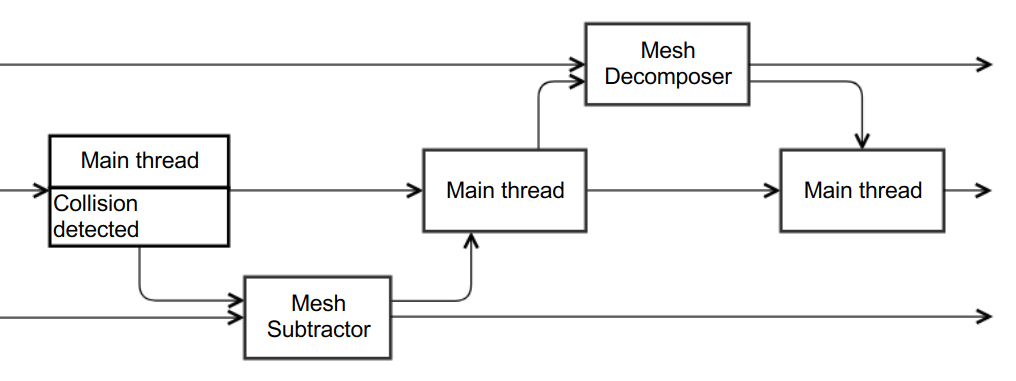
\includegraphics[width=\textwidth]{img/decompositionFlow}
        \caption{Diagram showing multiple threads handling collision event. }
        \label{fig:threads}
\end{figure}



\section{Collision handling}
\label{sec:collisions}


\section{Mesh Subtraction}
\label{sec:subtraction}

\section{Convex Decomposition}
\label{sec:decomposition}

\section{Data Representation}

